% study1.tex -- Section IV, Study 1 (writer W2, 2026-10-30). Binding contract: paper2-tnnls/SPEC.md v2.2.
% Sources: paper2/sections/{method,protocol,results}.tex (elsarticle draft; sentences follow SAP A4.2.2-A4.2.5), THEORY-ADDENDUM r1 R1.8
% (prop:snrcorr text), SAP A4.1.10 (Tier 3), A5.9 (family H prefix and placement), red-team REDTEAM-SPEC F1-F30 and V2-1.
% Rules kept here: I_j and S_G appear only in this section; no Study 2 symbol, role or result; no comparison word; the P discordance
% appears only as numbers in the P table (V2-1); family H only in its own subsubsection with the A5.9 prefix; Prop. 3 is not here.
% Every number carries a "% run:" comment with its file and key.

\section{Study 1: Masked-Likelihood Token Gating With Conformal Risk Control}\label{sec:study1}
Study~1 answers Q1 (\cref{sec:intro}); its object of measurement is an input-level source-validation gate, fixed before any test item
was seen.

\subsection{Method}\label{sec:study1-method}

\paragraph*{Suspicion score}
The $m=1\,024$ image positions are split at random into $K$ complementary groups, which define the caption-masked scores $B_j$ and
$D_j$ of \cref{sec:setting-evidence}.
% run: runs/P2-GATE-M2/threshold.json:K (= 8)
The gate uses $K=8$ and the suspicion
\begin{equation}
u_j=D_j-B_j ,
\label{eq:suspicion}
\end{equation}
where a larger $u_j$ marks a token whose observed code is less probable given the rest of the image than given its position alone.
The score never sees a caption, so the hypothesis under test cannot enter the gate, and no statement about its detection power is made
(supplement S-I).

\paragraph*{Threshold by conformal risk control}
The threshold is set on a calibration set $\mathcal D_{\rm cal}$ of $n_{\rm cal}$ clean pairs, disjoint by image from every other fold.
For item $i$ with suspicions $u_{ij}$, the false-alarm proportion at threshold $\tau$ is
\begin{equation}
L_i(\tau)=\frac1m\sum_{j=1}^{m}\ind\big[u_{ij}>\tau\big]\in[0,1],
\label{eq:loss}
\end{equation}
which does not increase in $\tau$.
With $\widehat F_{\rm cal}(\tau)=n_{\rm cal}^{-1}\sum_iL_i(\tau)$, the threshold is
\begin{equation}
\hat\tau=\inf\Big\{\tau:\ \tfrac{n_{\rm cal}}{n_{\rm cal}+1}\,\widehat F_{\rm cal}(\tau)+\tfrac1{n_{\rm cal}+1}\le\alpha\Big\},
\label{eq:crc}
\end{equation}
with $\hat\tau=+\infty$ if the set is empty; ties from \texttt{bf16} logits are broken by a small random jitter (supplement S-I).
% run: runs/P2-GATE-M2/threshold.json:n_cal (= 300); thresholds.0.05.alpha (primary level)
The calibration set has $n_{\rm cal}=300$ pairs and the primary level is $\alpha=0.05$.

\begin{proposition}[conformal risk control applied]\label{prop:crc}
Let the calibration items and a new clean test item be exchangeable as items, and let $L_i$ be given by \cref{eq:loss} with scores that
have no ties. Then $\E\big[L_{\rm test}(\hat\tau)\big]\le\alpha$.
\end{proposition}
\noindent\emph{Proof.} The loss is bounded by one and does not increase in the threshold, so the statement is Theorem~1 of conformal
risk control~\cite{angelopoulos2024crc} with bound $B=1$. \qed

This is the only guarantee in the paper, and it applies only to the expected share of flagged tokens in a clean test pair exchangeable
with the calibration pairs, which is at most $\alpha$.
The bound is over items, so tokens inside an item need not be exchangeable, and it is marginal over the draw of the calibration set.
It says nothing about detection power, about false alarms among the clean tokens of a corrupted item, or about a shift between
calibration and test.

\paragraph*{The gate and GATE-M}
Let $I_j=\ind[u_j\le\hat\tau]$ be the keep indicator of token $j$ and $G=\{j:I_j=0\}$ the flagged set.
GATE-M withholds the flagged tokens by masking them.
Because the logits of the image-direction passes do not depend on the image (\cref{sec:setting-evidence}), withholding token $j$ removes
its term $\Delta_j$ from the evidence:
\begin{equation}
S_{\rm G}=\sum_{j=1}^{m}I_j\Delta_j,\qquad Y_{\rm G}=\ind\big[S_{\rm G}>0\big],
\label{eq:gated}
\end{equation}
with a tie or an empty kept set counted as wrong.
With $I_j\equiv1$ this is the unweighted rule of \cref{sec:setting}, called \emph{none} below.
For a Bayes-optimal denoiser of the absorbing-state objective, masking $G$ marginalises it~\cite{ou2025radd}, but $G$ is selected from
the observed values, so the missingness is informative~\cite{rubin1976inference}.
Marginalising is then the Bayes answer only if no kept token is corrupted, corrupted values carry no information about clean ones,
corruption locations do not depend on the content, and the clean tokens in $G$ carry no evidence; this was stated in advance and is not
an account of any result.

Two further arms use the same flags.
A re-infilling arm re-infills the flagged tokens with the model, caption masked, and keeps the best of four unguided draws by chain log-likelihood,
with the sampler fixed in the analysis plan, not that of the backbone's authors.
The text direction, used only by family~B, scores the caption tokens with the image visible, minus the same pass with the image masked.

\paragraph*{A model of when withholding helps an additive statistic}
The following is theory under stated assumptions, not validated on UniDisc, and no result below is read through it.
Let a fraction $\rho$ of the $m$ tokens be corrupted.
Clean terms $\Delta_j$ have mean $\mu$ and variance $\sigma^2$ and are kept with probability $1-\phi_0$; corrupted terms have mean
$\mu_c$ and variance $\sigma_c^2$ and are kept with probability $1-\phi_1$.

\begin{lemma}[independent tokens]\label{lem:meanvar}
If the terms $\Delta_j$ are independent given the corruption labels and every $I_j$ is independent of all $\Delta_k$, then
\begin{align}
\E S_{\rm G}&=m\big[(1-\rho)(1-\phi_0)\mu+\rho(1-\phi_1)\mu_c\big],\label{eq:mean}\\
\Var S_{\rm G}&=m\Big[(1-\rho)\big\{(1-\phi_0)\sigma^2+\phi_0(1-\phi_0)\mu^2\big\}\notag\\
&\qquad+\rho\big\{(1-\phi_1)\sigma_c^2+\phi_1(1-\phi_1)\mu_c^2\big\}\Big].\label{eq:var}
\end{align}
For $\mu_c=0$ and $\E S_{\rm G}>0$, the gate raises $\E S_{\rm G}/\sqrt{\Var S_{\rm G}}$ above its value at $\phi_0=\phi_1=0$ if and only if
\begin{equation}
\rho\,\sigma_c^2\,(\phi_1-2\phi_0+\phi_0^2)\;>\;\phi_0(1-\phi_0)(1-\rho)\,(\sigma^2+\mu^2).
\label{eq:snr}
\end{equation}
\end{lemma}
\noindent\emph{Proof.} $\Var(I_j\Delta_j)=k\sigma_z^2+k(1-k)\mu_z^2$ with $k$ the keep probability of the token's class; sum over
tokens. The condition is \cref{prop:snrcorr} below at zero correlation. \qed

Three consequences follow.
A necessary condition is $\phi_1>2\phi_0-\phi_0^2$; a random gate, with $\phi_1=\phi_0$, lowers the ratio; and on a clean item any gate
with $\phi_0>0$ lowers it slightly.
The descriptive family E-pred uses \cref{eq:mean,eq:var} as preregistered.

\paragraph*{Correlated tokens}
Neighbouring image tokens are correlated, so \cref{eq:var} is an approximation.
The following statement replaces independence by an exchangeable correlation; it is theory under stated assumptions and is not
evaluated on the model.

\begin{proposition}[withholding with exchangeably correlated tokens]\label{prop:snrcorr}
Condition on the corruption labels, so that $(1-\rho)m$ tokens are clean and $\rho m$ are corrupted, with the moments and keep
probabilities of \cref{lem:meanvar}.
Assume (a) that for $j\neq k$ the correlation of $\Delta_j$ and $\Delta_k$ is $\gamma_0$ if both tokens are clean, $\gamma_1$ if both are
corrupted and $\gamma_{01}$ otherwise, with values for which the covariance matrix is positive semi-definite; and (b) that the keep
indicators $I_j$ are independent of each other and of every $\Delta_k$.
Then $\E S_{\rm G}$ is given by \cref{eq:mean}, and
\begin{equation}
\begin{aligned}
\Var S_{\rm G}={}&V+(1-\rho)m\big((1-\rho)m-1\big)(1-\phi_0)^2\gamma_0\sigma^2\\
&+\rho m(\rho m-1)(1-\phi_1)^2\gamma_1\sigma_c^2\\
&+2\rho(1-\rho)m^2(1-\phi_0)(1-\phi_1)\gamma_{01}\sigma\sigma_c,
\end{aligned}
\label{eq:varcorr}
\end{equation}
where $V$ is the right side of \cref{eq:var}.
If moreover $\mu_c=0$ and $\E S_{\rm G}>0$ with and without the gate, the gate raises $\E S_{\rm G}/\sqrt{\Var S_{\rm G}}$ if and only if
\begin{equation}
\begin{aligned}
&\rho\,\sigma_c^2\Big[(\phi_1-2\phi_0+\phi_0^2)\\
&\qquad+(\rho m-1)\,\gamma_1\,(\phi_1-\phi_0)(2-\phi_0-\phi_1)\Big]\\
&\quad+2\rho(1-\rho)\,m\,\gamma_{01}\,\sigma\sigma_c\,(1-\phi_0)(\phi_1-\phi_0)\\
&\qquad>\;(1-\rho)\,\phi_0(1-\phi_0)\,(\sigma^2+\mu^2).
\end{aligned}
\label{eq:snrcorr}
\end{equation}
Consequently:
(i) $\gamma_0$ does not enter \cref{eq:snrcorr}, and at $\gamma_1=\gamma_{01}=0$ it is \cref{eq:snr};
(ii) a gate with $\phi_1=\phi_0$, such as a random gate, lowers the ratio for every admissible correlation, and if $\gamma_{01}\ge0$ every
gate with $\phi_1\le\phi_0$ lowers it;
(iii) where $\phi_1>\phi_0$, a larger $\gamma_1$ or $\gamma_{01}$ can only turn a decrease of the ratio into an increase, so positive
correlation among corrupted tokens, or between clean and corrupted tokens, enlarges the region of $(\phi_0,\phi_1)$ in which the gate
raises the ratio, and as $(\rho m-1)\gamma_1\to\infty$ that region tends to $\{\phi_1>\phi_0\}$;
(iv) if $\gamma_{01}<0$, a gate that flags only clean tokens can raise the ratio;
(v) unlike \cref{eq:snr}, the condition depends on $m$.
\end{proposition}

\noindent\emph{Proof sketch.} Each of the $m(m-1)$ ordered pairs of distinct tokens adds $\E I_j\,\E I_k\,\mathrm{Cov}(\Delta_j,\Delta_k)$ to
$\Var S_{\rm G}$, which gives the three correlation terms of \cref{eq:varcorr}.
With $\mu_c=0$ the gate multiplies $\E S_{\rm G}$ by $1-\phi_0$, so it raises the ratio if and only if
$(1-\phi_0)^2\,\Var S_{\rm G}|_{\phi_0=\phi_1=0}>\Var S_{\rm G}$; the clean-pair terms scale by $(1-\phi_0)^2$ on both sides and cancel, and the
remaining terms, divided by $m$, give \cref{eq:snrcorr}.
The full proof is in supplement S-II. \qed

\Cref{fig:frontier} draws the frontier of \cref{eq:snrcorr}.
The ratio in \cref{prop:snrcorr} is the signal-to-noise ratio of the sum.
If the per-token terms are jointly Gaussian, the accuracy $P(S_{\rm G}>0)$ given the flags is $\Phi$ of the conditional ratio, which the
unconditional ratio approximates; without joint Gaussianity no statement about accuracy follows, and a gate can raise the ratio while
lowering the accuracy.
Assumption (b) is an approximation for this gate, whose flags are computed from the same token values as the evidence.
With correlation the ratio no longer grows like $\sqrt m$; it tends to a limit set by the shared component of the per-token terms.
E-pred does not use \cref{prop:snrcorr}, and the proposition is not used to interpret E-pred or any other result.

\begin{figure}[!t]
\centering
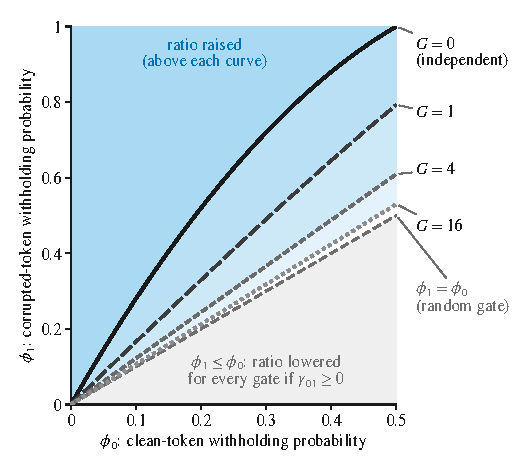
\includegraphics[width=\columnwidth]{figures/fig2_theory.pdf}
\caption{Model figure, no data: a model of when withholding helps an additive statistic (theory under stated assumptions, not validated
on UniDisc). Above each curve $\phi_1=b(\phi_0;G,\chi)$ of \cref{prop:snrcorr} (shaded), withholding raises
$\E S_{\rm G}/\sqrt{\Var S_{\rm G}}$; $\mu_c=0$, $\gamma_{01}=0$, $\chi=\rho\sigma_c^2/[(1-\rho)(\sigma^2+\mu^2)]=1$ and
$G=(\rho m-1)\gamma_1=0$ (independent tokens, \cref{eq:snr}), 1, 4 and 16. A larger $G$ lowers the curve toward the diagonal
$\phi_1=\phi_0$ (random withholding). Grey: every rule with $\phi_1\le\phi_0$ lowers the ratio when $\gamma_{01}\ge0$.}
\label{fig:frontier}
\end{figure}

\subsection{Preregistered Protocol}\label{sec:study1-protocol}
The protocol was fixed in a preregistration card, a statistical analysis plan with its addenda and a method specification before any
outcome of the main run existed; pins, audits, amendments and the protocol details omitted here are in supplement S-I.

\paragraph*{Folds and negatives}
% run: runs/P2-GATE-FOLDS (folds.json sizes and seed 20261029; 494 pilot image ids excluded)
Four image-disjoint sets were drawn from COCO val2017~\cite{lin2014coco} by image id with seed 20261029: calibration (300 pairs),
headroom (100), test (300, with an ordered extension to 500 if the sample-size rule asks for it) and the 200 items of an earlier
detection pilot, which form the detection set.
The 494 image ids of the two pilots are excluded from the new folds.
The wrong caption of an item is a caption of another image that shares no annotated COCO category with the true image, fixed once per
item and shared by every arm and corruption.

\paragraph*{Headroom rule and sample size}
Each realistic corruption has two severities (rungs), walked in order from the one defined in \cref{sec:setting-corruptions}.
Two sanity corruptions replace tokens by uniform random codes (one $8\times8$ patch of the token grid; 15\,\% of tokens) and form the
positive control.
On the 100 headroom items, with no gate flag computed, the first rung at which the size-normalised evidence falls under corruption and
recovers under the changed-code gate, which keeps exactly the tokens whose code did not change, is the operating point.
The largest headroom discordance $D^\ast$ between the changed-code gate and no gate then sets the test size by a pre-written rule.
The decision file was committed before the first test item was scored.

\paragraph*{Arms and controls}
The primary contrast is GATE-M against none.
The controls are a geometry-matched random gate (the flag mask shifted on the torus, three seeds), equal-size scattered and top-$k$ gates,
the changed-code gate, a pixel denoiser and GATE-M on clean images (supplement S-II).
Token detection is measured against changed-code labels by per-item AUROC.
Cheap rivals are admitted in both orientations, so the rival and its sign are chosen on the data; a one-pass observed-position score of
the non-finetuned backbone (TbV score~\cite{jhingran2026trustverify}) is reported beside them.

\paragraph*{Families and reading rules}
The primary family P has three hypotheses, one per realistic corruption at its operating point.
Each compares GATE-M with none on the paired correctness of \cref{eq:gated} by the exact two-sided McNemar test, with Holm correction over
three at familywise level 0.05; a corruption without an operating point stays in the family with $p=1$.
The wording for every outcome was fixed before the headroom decision was written.
The label is \emph{positive} if a hypothesis is rejected after Holm with $b>c$ and none with $c>b$.
It is \emph{negative} if none is rejected and, for every corruption with an operating point, the 90\,\% paired bootstrap interval of the
net accuracy change lies inside $(-0.05,+0.05)$ with at least 240 completed items; it is \emph{inconclusive} otherwise.
A null result is worded as a bounded change, never as an absence of effect.
The percentile interval has zero width whenever no pair is discordant (counts in \cref{tab:familyP}).
Each secondary family has its own level 0.05 (sizes, tests and wording rules in supplement S-I).
The positive control PS repeats the P test on the two sanity corruptions (Holm over two); a pass reads ``the pipeline is not broken''.
A mechanism test (GATE-M against the geometry-matched gate) and a second-model family run only on a corruption with a primary rejection
with $b>c$. \Cref{tab:glance} lists the families reported in the main text with their status; supplement S-II maps all of them.

\subsection{Results}\label{sec:study1-results}
Bootstrap intervals use 10\,000 resamples, accuracy is image-direction verification accuracy, a cell is bold only when its
preregistered test rejected, and there is no adjustment across families (\cref{sec:setting-tests}).

\subsubsection{Operating points and family P}
% run: runs/P2-GATE-M3/family.json:rungs.* (first rung passed for jpeg, noise, splice); n_rule.* (D_star 19, rule R2, test_fold 500)
The first rung of every realistic corruption passed the headroom rule, and $D^\ast=19$ selected 500 test items with the correctness
endpoint (supplement S-II gives the headroom statistics).
% run: runs/P2-GATE-M4/analysis.json:primary.per_corruption.{jpeg,noise,splice}.{delta,ci90,n}; outcome.label (= negative)
In the preregistered test no improvement was detected under JPEG quality~10, Gaussian noise with $\sigma=0.10$ or a $128$-pixel splice.
For each tested corruption the 90\,\% interval of the net accuracy change lay inside $\pm0.05$: $-0.002$ ($-0.006$ to $0.000$) under JPEG,
$0.000$ ($0.000$ to $0.000$) under noise and $-0.004$ ($-0.010$ to $0.002$) under splice, with $n=500$ each, so an improvement larger than
0.05 is excluded and a loss larger than 0.05 is excluded.
This does not show that the gate has no effect.
% D0097: scope wording of A4.2.2 item 7 tightened (category-disjoint negatives; exp_p2/gate/folds.py assign_negatives)
It holds in one pretrained unified masked diffusion model (UniDisc, 1.4B parameters) on COCO image-caption pairs with a random caption of
an image sharing no annotated COCO category (category-disjoint) as the negative, at one severity per corruption.
% run: runs/P2-GATE-M4/analysis.json:completeness.*; outcome.label
By the pre-stated rule the label of family P is \emph{negative}: no hypothesis was rejected after Holm correction over three, and every
corruption had an operating point and 500 completed items, with no caption-token exclusion and no empty or non-finite evidence.
\Cref{tab:familyP} gives the full test and \cref{fig:p_result} its intervals.

\begin{table*}[!t]
\centering
\caption{Family P: GATE-M Against No Gate on the 500 Test Items}
\label{tab:familyP}
\footnotesize
\setlength{\tabcolsep}{4pt}
\resizebox{\textwidth}{!}{% tab1_familyP.tex: generated by paper2-tnnls/scripts/tab1_familyP.py from committed runs/ files. Do not edit by hand.
% Family P only. Holm over three corruptions (m = 3); p: exact two-sided McNemar. The family label is negative (outcome.label); the abstract sentence is the preregistered one.
% Under noise b = c = 0: the bootstrap intervals are the single point zero (absence of discordant items, not a measured precision); the exact bound is the descriptive complement.
% Exact Clopper-Pearson bound: runs/P2-PAPER-BOUNDS/p_exact_bounds.json, 'added at writing, descriptive; not preregistered'; list it in the deviations box.
\begin{tabular}{@{}lrccrrrrll@{}}
\toprule
Cell & $n$ & Acc.\ none & Acc.\ GATE-M & $b$ & $c$ & $n_d$ & Net diff. & $p$ ($p_{\rm Holm}$) & Preregistered decision \\
\midrule
% run: runs/P2-GATE-M4/analysis.json primary.per_corruption.jpeg.{n,acc_a,acc_b,b,c,n_d,delta,p,p_holm}
P1: JPEG, quality 10 & 500 & 0.838 & 0.836 & 0 & 1 & 1 & $-0.002$ & 1.00 (1.00) & not rejected; 90\% interval inside $(-0.05,\,0.05)$ \\
% run: runs/P2-GATE-M4/analysis.json primary.per_corruption.jpeg.{ci90,ci95,ci9833}
% run: runs/P2-PAPER-BOUNDS/p_exact_bounds.json per_corruption.jpeg.{bound_abs_net_change_95}; meta.label
\multicolumn{10}{l}{\footnotesize intervals: 90\% $[-0.006,\,0.000]$;\; 95\% $[-0.006,\,0.000]$;\; 98.33\% $[-0.008,\,0.000]$;\; exact 95\% bound on $|$net change$|$ 0.011 (added at writing, descriptive)} \\
% run: runs/P2-GATE-M4/analysis.json primary.per_corruption.noise.{n,acc_a,acc_b,b,c,n_d,delta,p,p_holm}
P2: noise, $\sigma=0.1$ & 500 & 0.676 & 0.676 & 0 & 0 & 0 & 0.000 & 1.00 (1.00) & not rejected; 90\% interval inside $(-0.05,\,0.05)$ \\
% run: runs/P2-GATE-M4/analysis.json primary.per_corruption.noise.{ci90,ci95,ci9833}
% run: runs/P2-PAPER-BOUNDS/p_exact_bounds.json per_corruption.noise.{bound_abs_net_change_95}; meta.label
\multicolumn{10}{l}{\footnotesize intervals: 90\% $[0.000,\,0.000]$;\; 95\% $[0.000,\,0.000]$;\; 98.33\% $[0.000,\,0.000]$;\; exact 95\% bound on $|$net change$|$ 0.007 (added at writing, descriptive)} \\
% run: runs/P2-GATE-M4/analysis.json primary.per_corruption.splice.{n,acc_a,acc_b,b,c,n_d,delta,p,p_holm}
P3: splice, 128 px & 500 & 0.876 & 0.872 & 1 & 3 & 4 & $-0.004$ & 0.625 (1.00) & not rejected; 90\% interval inside $(-0.05,\,0.05)$ \\
% run: runs/P2-GATE-M4/analysis.json primary.per_corruption.splice.{ci90,ci95,ci9833}
% run: runs/P2-PAPER-BOUNDS/p_exact_bounds.json per_corruption.splice.{bound_abs_net_change_95}; meta.label
\multicolumn{10}{l}{\footnotesize intervals: 90\% $[-0.010,\,0.002]$;\; 95\% $[-0.012,\,0.004]$;\; 98.33\% $[-0.014,\,0.004]$;\; exact 95\% bound on $|$net change$|$ 0.020 (added at writing, descriptive)} \\
\bottomrule
\end{tabular}
}

\vspace{2pt}
\parbox{\textwidth}{\scriptsize $b$: items that GATE-M answers correctly and the ungated rule incorrectly; $c$: the reverse; $n_d=b+c$;
net difference $=(b-c)/n$. Paired percentile bootstrap intervals (10\,000 resamples) at 90\,\% (the level of the preregistered
decision), 95\,\% and 98.33\,\% (the Holm level of the smallest-$p$ step); zero width when $n_d=0$. $p$: exact two-sided McNemar;
$p_{\rm Holm}$: Holm over the three corruptions. The exact Clopper--Pearson 95\,\% bound on the absolute net change was added at
writing and is descriptive, not preregistered. No test rejected, so nothing is bold.}
\end{table*}

\begin{figure}[!t]
\centering
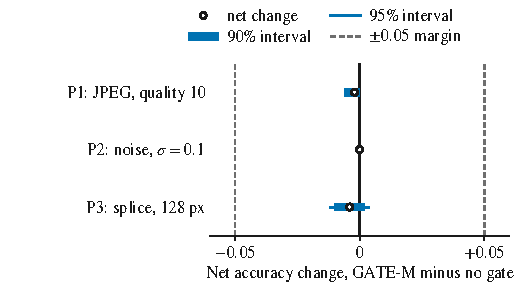
\includegraphics[width=\columnwidth]{figures/fig3_study1_P.pdf}
\caption{Family P: net accuracy change of GATE-M minus no gate (open circle), $n=500$ items per corruption (P1 JPEG quality 10, P2
Gaussian noise with standard deviation 0.1, P3 splice of 128 px). Thick bar: 90\,\%, thin bar: 95\,\% paired percentile bootstrap
interval (10\,000 resamples); solid line at 0; dashed lines: the $\pm0.05$ margin. An interval has zero width when no pair is
discordant (counts in \cref{tab:familyP}).}
\label{fig:p_result}
\end{figure}

\subsubsection{Calibration and the clean control}
% run: runs/P2-GATE-M4/analysis.json:calibration.fap_check.per_alpha.0.05.{F,ci_bootstrap,Z_cal}; critical_value (= 2.13)
On the 500 clean test pairs the realised flagged share was 0.0456 at $\alpha=0.05$ (95\,\% interval 0.0442 to 0.0470), with a calibration
statistic (the standardised excess of the flagged share over $\alpha$) of $-3.59$ against the violation bound of 2.13, so there is no
evidence of violation of \cref{prop:crc} (other levels in supplement S-II).
% run: runs/P2-GATE-M4/analysis.json:calibration.per_condition.*.fap_on_clean_tokens
The guarantee does not cover the unchanged tokens of corrupted items, whose flagged share was 0.036 to 0.044 under the realistic
corruptions and 0.089 under swap (supplement S-II).
% run: runs/P2-GATE-M4/analysis.json:s_c.{acc_a,acc_b,delta,ci95,p}
In the clean control GATE-M gave 0.882 against 0.880 without a gate (net $0.002$, 95\,\% interval $-0.004$ to $0.010$; $p=1.00$): no change
was detected.

\subsubsection{Positive control (PS, pipeline check)}
% run: runs/P2-GATE-M4/analysis.json:ps.per_corruption.patch.{acc_a,acc_b,delta,ci95,p,p_holm}; ps.per_corruption.swap.{acc_a,acc_b,delta,ci95,p,p_holm} (values as printed in tables/tab_ps.tex)
On the 500 test items GATE-M gave 0.870 against 0.870 without a gate under the patch corruption (net 0.000, 95\,\% interval $-0.008$ to
0.008; $p=1.00$, Holm-adjusted 1.00) and 0.876 against 0.870 under swap (net 0.006, $-0.008$ to 0.020; $p=0.581$, Holm-adjusted 1.00).
% run: runs/P2-GATE-M4/analysis.json:ps.positive_control (= not met)
Neither hypothesis of the positive control was rejected (full table in supplement S-II), so the control was not met, which by the plan
reads ``pipeline defect suspected, audit triggered''.
% run: runs/P2-A23-AUDIT/a23_ps_audit.json (recomputation of every PS quantity, 0 mismatches); unit-test count (584 passed, 5 skipped,
% 0 failed): runs/P2-A23-AUDIT audit record, research/paper2/prereg/A2.3-AUDIT-PS-2026-10-29.md line 75 (pointer per D0100; number audit M6)
The plan's audit (an automated audit run in the authors' own pipeline, not an independent review) ran the unit tests of the run's code (584 passed, 5 skipped, none
failed), read the code path of PS and recomputed every PS quantity from the stored arrays of all 500 items; it found no defect and
changed nothing, and since a recomputation cannot see an error upstream of the stored arrays, it is not read as a check of the whole
pipeline.

\subsubsection{Token detection}
% run: runs/P2-GATE-M1/analysis.json:table.{patch,swap}.q.{mean,lo,hi}; table.{jpeg,noise}.q.n (= 197, 198; n_items = 200)
On the detection items (about 200; \cref{tab:detection} gives the exact count per corruption) the gate's masked-likelihood score
$q_j=-u_j$ separates code-level random replacements but is near chance on JPEG and Gaussian noise.
% run: runs/P2-GATE-M1/analysis.json:table.{jpeg,noise}.{q,tbv}.{mean,lo,hi}
On noise it is below the one-pass TbV score of the non-finetuned backbone; the marginal intervals do not overlap, which is descriptive,
and no paired test was run; on JPEG the two overlap.
% run: runs/P2-GATE-M4/analysis.json:s_d2.per_corruption.{jpeg,noise}.{diff_mean,ci95,p_holm,n_eligible}
The best cheap rival, the pixel variance of a token's patch with its sign reversed, was frozen and the contrast repeated on the test
items: $q$ minus the rival was $-0.198$ ($-0.211$ to $-0.186$; 492 items) under JPEG and $-0.258$ ($-0.267$ to $-0.250$; 497 items)
under noise, with Holm-adjusted $p=0.0004$ (the resolution floor of 10\,000 resamples).
% run: runs/P2-GATE-M1/analysis.json:paired_q_vs_best_cheap.{jpeg,noise}.{best_cheap,rival_sign,diff_mean,ci95,p_holm}; table.*.tex_neg
On the detection items, where the rival and its sign were selected, $q$ also lies below it (same-item selection; \cref{tab:detection}).
The preregistered falsifier for the score was therefore met, and this paper makes no claim that the score detects corrupted codes more
accurately than cheap methods.
The labels mark codes that the tokeniser changed, which a texture score can anticipate without any reference to the evidence; the
rival's win is read as this label-circularity concern, not as an account of any corruption effect.

\begin{table*}[!t]
\centering
\caption{Detection of Changed Image Tokens on the Detection Items: Per-Item AUROC}
\label{tab:detection}
% run: runs/P2-GATE-M1/analysis.json:paired_q_vs_best_cheap.{jpeg,noise}.p_holm (= 0.0004)
\footnotesize
\resizebox{\textwidth}{!}{% tab_detection.tex: generated by paper2-tnnls/scripts/tab_detection.py from committed runs/ files. Do not edit by hand.
% AUROC against changed-code labels per item; 95% percentile bootstrap over items (10000 resamples); rival and its sign chosen on these data (sign oracle): rival values optimistic.
% bold: Holm-adjusted p < 0.05 of the paired contrast (JPEG, noise); no claim about detection relative to any rival.
\begin{tabular}{@{}lrllll@{}}
\toprule
Corruption & Items & $q$ (AUROC) & TbV score, one pass (AUROC) & Best cheap rival, sign (AUROC) & $q$ minus rival \\
\midrule
% run: runs/P2-GATE-M1/analysis.json table.patch.{q,tbv,plainB}.{mean,lo,hi,n}; paired_q_vs_best_cheap.patch.{best_cheap,rival_sign,diff_mean,ci95,p_holm}
Patch, $8\times8$ codes & 200 & 0.961 $[0.959,\,0.963]$ & 0.854 $[0.847,\,0.861]$ & plain $B$ ($+$): 0.964 $[0.962,\,0.966]$ & $-0.003$ $[-0.004,\,-0.003]$ \\
% run: runs/P2-GATE-M1/analysis.json table.swap.{q,tbv,plainB}.{mean,lo,hi,n}; paired_q_vs_best_cheap.swap.{best_cheap,rival_sign,diff_mean,ci95,p_holm}
Swap, 15\% of codes & 200 & 0.955 $[0.952,\,0.957]$ & 0.859 $[0.854,\,0.864]$ & plain $B$ ($+$): 0.960 $[0.958,\,0.962]$ & $-0.005$ $[-0.006,\,-0.005]$ \\
% run: runs/P2-GATE-M1/analysis.json table.jpeg.{q,tbv,tex_neg}.{mean,lo,hi,n}; paired_q_vs_best_cheap.jpeg.{best_cheap,rival_sign,diff_mean,ci95,p_holm}
JPEG, quality 10 & 197 & 0.561 $[0.547,\,0.575]$ & 0.581 $[0.569,\,0.593]$ & patch texture ($-$): 0.756 $[0.743,\,0.768]$ & $-0.195$ $[-0.214,\,-0.175]$ \\
% run: runs/P2-GATE-M1/analysis.json table.noise.{q,tbv,tex_neg}.{mean,lo,hi,n}; paired_q_vs_best_cheap.noise.{best_cheap,rival_sign,diff_mean,ci95,p_holm}
Noise, $\sigma=0.1$ & 198 & 0.503 $[0.493,\,0.513]$ & 0.607 $[0.597,\,0.618]$ & patch texture ($-$): 0.768 $[0.760,\,0.776]$ & $-0.265$ $[-0.278,\,-0.253]$ \\
\bottomrule
\end{tabular}
}

\vspace{2pt}
\parbox{\textwidth}{\scriptsize Mean per-item AUROC against changed-code labels, 95\,\% percentile bootstrap intervals over items
(10\,000 resamples). $q$: the gate's score; TbV score: one-pass observed-position score of the non-finetuned model; rival: the best
cheap score in either orientation, chosen on these data (same-item selection, so optimistic), with its sign. Items: detection items
entering each row. Last column: paired difference $q$ minus rival (Holm-adjusted $p=0.0004$ for JPEG and noise).}
\end{table*}

\subsubsection{Mechanism and the remaining secondary families}
% run: runs/P2-GATE-M4/analysis.json:s_m.per_corruption.{jpeg,noise,splice}.tested (all false)
The mechanism test tested no hypothesis and the second-model family was not run, because both are gatekept by a primary rejection with
$b>c$.
% run: runs/P2-GATE-M4/analysis.json:mechanism.{jpeg10,noise0.1,splice128}.y.*, s_z.*, s_dn.*; edec.json; epred_score.json; P2-GATE-M5/coherence.json
The equal-size gates, the evidence-ratio and pixel-denoising families, the descriptive families (including E-pred) and the denoiser's
coherence check are in supplement S-II and enter no statement about P.

\subsubsection{Re-infilling the flagged tokens}
% run: runs/P2-GATE-S2/analysis.json:per_cell.{patch,splice}.{n,delta,ci95,p_holm,reading}; completeness.completed_n (= 300)
On 300 items per cell, as planned, re-infilling the flagged set against re-infilling an equal-size random set (kept draw, exact
McNemar, Holm over two) gave a net change of $0.010$ ($0.000$ to $0.023$; $p_{\rm Holm}=0.50$) under the patch corruption and $-0.003$ ($-0.017$ to $0.007$; $p_{\rm Holm}=1.00$) under
splice.
Neither cell was rejected; there is no evidence that the flagged set is better placed than a random one under this sampler, and nothing
is stated about the backbone's own re-infilling.

\subsubsection{Family B: the two directions on foil captions}
Family~B, the preregistered two-way fusion test, compares a score-level combination of the text and image directions (Fisher
discriminant weights fitted on separate fit pairs and frozen) with the better single direction.
Its pairs come from FOIL-COCO~\cite{shekhar2017foil}, clean images whose negative caption differs from the true caption in one word, so it
is not a corruption test.
% run: runs/P2-GATE-FOIL/analysis.json:test.{n,acc_a,acc_b,delta,ci95,p}; combination_beat_best_single (= false); analysed at commit 10e6bc0f
On the 298 test pairs the combination reached 0.876 against 0.879 for the better direction, the text direction (net $-0.003$, 95\,\%
interval $-0.010$ to $0.000$; $p=1.00$), so no gain of the combination over the better single score was detected (fit pairs and
minimum detectable gain in supplement S-II).

\subsubsection{Family H (added after the primary result)}\label{sec:study1-H}
% run: runs/P2-GATE-H3/family.json:n_headroom_items (= 50); n_rule.h_rule (= H-NOGO); n_rule.G_max_headroom (= null); go (= false)
In a separately labelled family added after the primary result was known (family H: SugarCrepe hard
negatives~\cite{hsieh2023sugarcrepe} on 50 COCO images not used elsewhere; Holm over the
same three corruptions), the pre-written pilot rule found no corruption with decision headroom on 50 pilot images, so the family's test
was not run.
Its rules and code were committed before any hard-negative item was scored (disclosure, caveats and decision record in supplement
S-III), and because its test was not run, nothing is stated about the gate on hard negatives.

\subsubsection{Exploratory analyses}
% run: runs/P2-GATE-M4/tier3_fusion.json:cells.*.contrasts.*_minus_GM (72 intervals; run once after analysis.json was committed)
An exploratory comparison pre-specified in an addendum to the analysis plan, with intervals only and run once after the primary
analysis was committed, contrasts the hard gate with five combiners of the same $\Delta_j$: three that need no detector, a discount of
the flagged tokens, and a graded weight on every token.
% run: runs/P2-GATE-M4/tier3_fusion.json:cells.noise0.1.arms.{GM,MED,TM20}.acc (= 0.676, 0.678, 0.682); cells.noise0.1.contrasts.{MED,TM20}_minus_GM.{ci95,reading} (not_distinguishable); cells.{jpeg10,splice128}.contrasts.{MED,TM20}_minus_GM.reading (= below)
% (number audit M1: the earlier sentence "no detector-free combiner gave higher verification accuracy than the hard gate" contradicted the noise cell)
The median and 20\,\% trimmed-mean combiners are reported with their exact intervals in supplement S-II.
% run: runs/P2-GATE-M4/tier3_fusion.json:cells.{jpeg10,noise0.1,splice128}.contrasts.TM-G_minus_GM.{n_d,discordance_bound_B,counts_against}
The data do not show a difference between the hard gate and a trimmed mean that removes as many tokens as the gate flagged (exact 95\,\%
bounds on the difference of 0.023, 0.014 and 0.017).
By the pre-stated rule, this counts against the added value of the detector on those cells (every cell, comparator and limit in
supplement S-II).
% run: runs/P2-GATE-SUITE/analysis.json:cells.*.gm_vs_none.ci95 (8 cells, 100 items each; every interval contains 0)
In an exploratory suite of eight further cells (four corruption types of the imagecorruptions package~\cite{michaelis2019imagecorruptions}
at two severities, 100 test items each; intervals only), no cell's 95\,\% interval of GATE-M minus none excluded zero (supplement S-II).

\subsubsection{Cost}
% run: runs/P2-GATE-M4/items.jsonl:n_rows, seconds, peak_gb (median 84 rows, 11.2 s, max 8.2 GB)
The main-test pass, which computes every arm of Study~1 at once, used a median of 84 network rows and 11.2~s per item on one
12~GB laptop GPU, with a peak memory of 8.2~GB (supplement S-II).
